% Appendix A

\chapter{TopFCNH} % Main appendix title

\label{AppendixB} % For referencing this appendix elsewhere, use \ref{AppendixA}

% outline
%----------------------------------------------------------------------------
% 
%
\section{Introduction}

Besides my work on the Fast Calorimeter Simulation Challenge, I have also been involved in the TopFCNH project. For the sake of better understanding the concept and workflow of an analysis. This project aims to study the the interaction between top quark, higgs boson, and a light quark (u or c) in the context of the Standard Model Effective Field Theory (SMEFT) and search for new physics phenomena. It's just at the beginning stage, so what I have done includes roundtable presentation, gridpack preparation, monte carlo and data comparison. In this appendix, I will provide an overview of the TopFCNC project, the analysis workflow, gridpack generation, and the current status of the project.

\section{Background}

While higgs boson has been discovered in 2012, which is the newest particle, and the LHC is mainly designed for observing it, the top quark is the heaviest known elementary particle in the Standard Model (SM). The interaction between top quark and higgs boson is of great interest, as it can provide many insights into many unknown field.

The top-quark flavor-changing neutral current (TopFCNC) decay $t \to Hq$ (where $q = u, c$) is highly suppressed in the Standard Model (SM) due to the Glashow-Iliopoulos-Maiani (GIM) mechanism. \cite{maiani_gim_2013} The predicted SM branching ratio for this process is $BR(t \to Hq) \sim 10^{-15} - 10^{-13}$, making it practically unobservable at the LHC. However, many beyond-the-SM (BSM) theories predict significantly enhanced branching ratios, making it a promising channel for new physics searches. As you can see the figure \ref{fig:TopFCNC}

\begin{figure}[htbp]
    \centering
    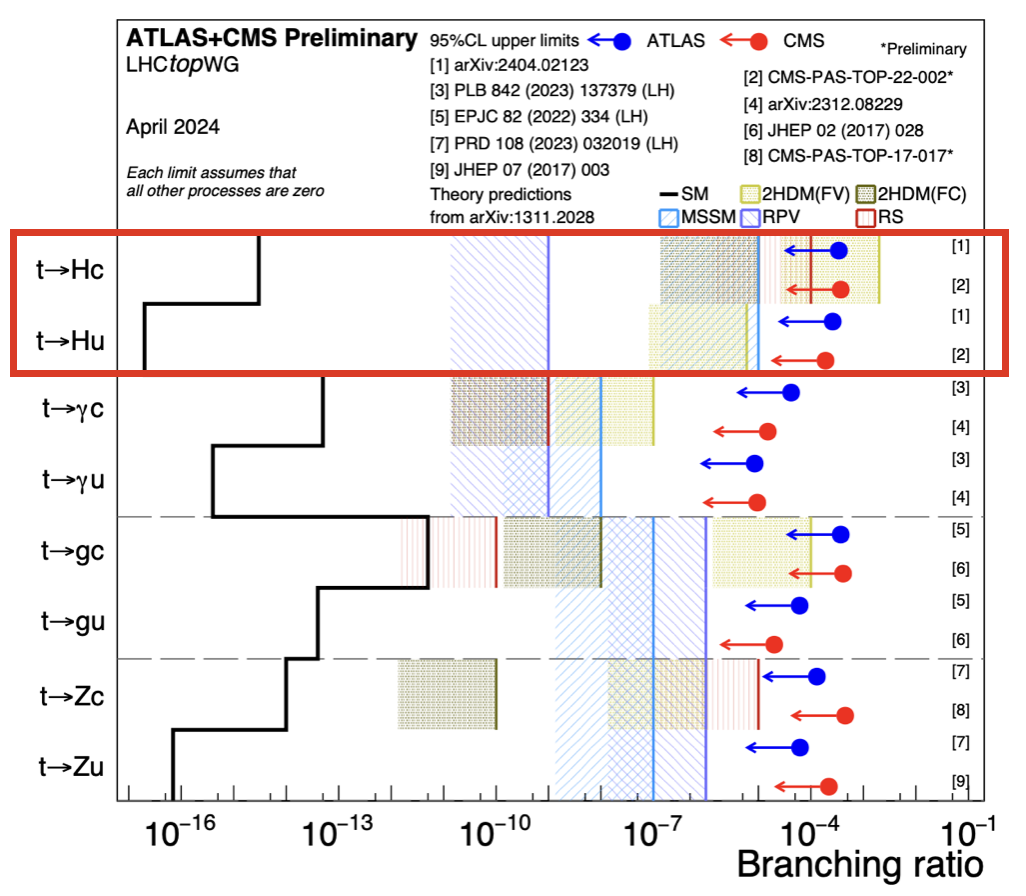
\includegraphics[width=0.8\textwidth]{Figures/topfcnc.png}
    \caption{The prediction and the result so far}
    \label{fig:TopFCNC}
\end{figure}

Several BSM frameworks predict an increase in the branching ratio. The Two-Higgs Doublet Model (2HDM) suggests that $BR(t \to Hq)$ could reach $10^{-5} - 10^{-3}$.\cite{noauthor_fcnchistory_nodate} Similarly, Supersymmetric Models (SUSY) predict comparable enhancements. Additionally, theories involving a Composite Higgs and Extra Dimensions indicate the possibility of increasing the branching ratio to $10^{-4} - 10^{-3}$. Given these enhancements, detecting $t \to Hq$ at the LHC would be a clear sign of new physics.

Among the Higgs boson decay channels, the $H \to \gamma\gamma$ (diphoton decay) is particularly attractive due to its clean experimental signature in the CMS electromagnetic calorimeter. The branching ratio of $H \to \gamma\gamma$ for a 125 GeV Higgs is approximately $0.2\%$, which is small but provides a well-reconstructed final state. Our research focuses on the process $pp \to t\bar{t}, t \to Hq, H \to \gamma\gamma$, where the diphoton final state can be efficiently detected using high-resolution electromagnetic calorimetry.

Photon triggers in CMS have high efficiency, with single-photon triggers reaching efficiencies above $99\%$ and double-photon triggers capturing over $88\%$ of events. Major backgrounds include prompt diphoton production ($pp \to \gamma\gamma + \text{jets}$) and fake $\gamma + j $, which can be reduced by later analysis methods.

\section{Analysis Workflow}
\section{Gridpack Generation}
\section{Current Status}